\documentclass[fleqn, final]{../styles/unmphythesis}
\usepackage{../styles/qxd}
\renewcommand{\thechapter}{2}
%\newcommand{\thechapter}{1}

\makeindex
\begin{document}

%<*atomicphysicsformulas>

\chapter{Some useful formulas of atomic physics}\label{chap:summaryofatomicphysicsformulas}
We summarize some useful formulas for atoms presented in vacuum (including inside an optical cavity) in this appendix for us to generalize without proving some concepts for the nanophotonic waveguide case. We collect the formulas in various sources, which include but not limited to Refs.~\cite{Deutsch2010a,Kimble1998,Baragiola2014Open,Norris2014,Steck2007Quantum}.

\section{Spontaneous atomic decays}
Scalar polarizability of an atom:
\begin{align}
\alpha &=-\frac{|d_{eg}|^2}{\hbar (\Delta+i\Gamma/2)}, \,\, (\Delta=\omega-\omega_{eg}\equiv \omega-\omega_0),
\end{align}
where $ d_{eg} $ denotes the atomic momentum due to the dipole oscillations between $ \ket{g} $ and $ \ket{e} $ states, and $ \Gamma $ is the decay rate of the atom. In the dispersive interaction regime, one can usually ignore the imaginary part of the atomic polarizability as $ \Delta\gg \Gamma $~\cite{Deutsch2010a}, and hence
\begin{align}
\alpha \approx -\frac{|d_{eg}|^2}{\hbar\Delta}.
\end{align}

Decay rates (natural linewidth) of an atom in vacuum:
\begin{align}\label{eq:naturallinewidth}
\Gamma_{vac}=\Gamma_0 &= \frac{4}{3} \left( \frac{\omega_0}{c}\right)^3 \frac{|d_{eg}|^2}{\hbar}
\end{align}

When the atom is placed in a Gaussian laser field, the decay rate of the atom could be modified as
\begin{align}
\Gamma^{1D} &= \Gamma_g=2\pi \frac{|d_{eg}|^2}{\hbar A_{e\!f\!f}}\left(\frac{\omega_0}{c} \right),
\end{align}
where the scripts $ 1D $ and $ g $ indicate the effect is caused by the coupling to a quasi-1D propagating light field (guided), and $ A_{e\!f\!f} $ is the effective mode area of the beam. For commonly used atomic traps in free space, the TEM$_{00} $ mode is employed to probe atoms, which has an effective mode area given by
\begin{align}
A_{e\!f\!f} &= \frac{A}{|\mathbf{u}_{00}(\br')|^2}=\frac{A}{|\mathbf{u}_{00}(r'_\perp)|^2},
\end{align}
where $ \mathbf{u}_{00}(\br) $ is the TEM$_{00}$ mode of the Gaussian beam (see Appendix~\ref{chap:paraxialapproximation}), and $ A=\pi w_0^2/2 $ is the mode area at the $ z=0 $ plane with $ w_0 $ the waist radius of the mode. 

We define the resonant cross section of an atom to be
\begin{align}
\sigma_0 &= \frac{3\lambda^2}{2\pi}=\frac{6\pi}{k_0^2}=\frac{6\pi c^2}{\omega_0^2},
\end{align}
and then the decay rate due to the coupling to the laser beam can be rewritten as
\begin{align}\label{Gamma1DGammavac_appendix}
\Gamma^{1\!D} &= \frac{1}{4} \frac{\sigma_0}{A_{e\!f\!f}}\Gamma_0.
\end{align}
On the other hand, due to the dispersive interaction from the atom, the optical mode of the input TEM$_{00}$ Gaussian laser beam will also yield a phase shift, $ \delta \phi $, given by
\begin{align}
\delta\phi &=2\pi \frac{\omega_0}{c A_{e\!f\!f}} \re[\alpha] = 2\pi \frac{\omega_0}{cA} \re[\alpha] |\mathbf{u}_{00}(\br')|^2 =-\frac{1}{A} \sigma_0 |\mathbf{u}_{00} (r'_{\!\perp})|^2 \frac{\Gamma_{vac}}{4\Delta},
\end{align}
We can also write 
\begin{align}\label{phaseshiftGamma1D}
\delta\phi &= -2\pi \frac{|d_{eg}|^2}{\hbar \Delta} \frac{\omega_0}{cA_{e\!f\!f}}=-\frac{\Gamma^{1\!D}}{\Delta}.
\end{align}

In calculating the dipole moment of an atom, we use Eq.~\eqref{eq:opdmm'} based on the Wigner-Eckart theorem to define the dipole moment amplitude of $ \hat{\mathbf{d}}_q $ by~\cite{Deutsch2010a}
\begin{align}
&\quad \bra{j'f'm'}\hat{\mathbf{d}}_q\ket{jfm} = o_{jf}^{j'f'}C_{f'm'}^{f,m;1,q} \bra{j'}\lvert d\rvert\ket{j}\\
&= (-1)^{f'+i+j'+1}\sqrt{(2j'+1)(2f+1)}\left\{ 
\begin{array}{ccc}
	f' & i & j' \\
	j & 1 & f
\end{array}\right\}C_{f'm'}^{f,m;1,q} \bra{j'}\lvert d\rvert\ket{j},
\end{align}
where we denote $ i $ as the nuclear spin number, $o_{jf}^{j'f'}$ as the relative oscillator strengths, $C_{f'm'}^{f,m;1,q}$ as the Clebsch-Gordan coefficients, and $\bra{j'}\lvert d\rvert\ket{j}$ as the reduced dipole matrix elements. 
Note that different research groups may define the transition amplitudes of the dipole operator in their own conventions, which leads to inconsistent definitions of the reduced matrix elements in literature.
In this dissertation, we can calculate the reduced matrix elements using the experimentally measured partial lifetimes, $ \tau_{j'\!j} $, due to spontaneous emissions from $ j' $ to $ j $~\cite{Ding2012Corrections,McKeever2004,Arora2007Magic} by 
\begin{align}
|\bra{j'}\lvert d\rvert\ket{j}|^2 = \frac{3\pi \epsilon_0\hbar c^3}{\omega_{j'\!j}^3\tau_{j'\!j}},\label{eq:reducedmatrixelements}
\end{align}
where $ \epsilon_0 $ is the dielectric constant of vacuum, and $ \omega_{j'\!j} $ is the resonance frequency of the $ j'\rightarrow j $ transition.
Note, here we use the convention for the reduced dipole matrix element given by Wigner~\cite{Wigner1959Group} and Rose~\cite{Rose1957Elementary}.
Whilst, Refs.~\cite{Ding2012Corrections} and~\cite{LeKien2013} by Ding, Kimble, Le Kien, Rauschenbeutel, \textit{et al.}, for example, use the convention of Racah~\cite{Racah1942Theory,Fano1959Irreducible} and Edmonds~\cite{Edmonds1957Angular}.
Their definition of the reduced matrix elements' square is $ (2j'+1) $ times greater than ours. Ref.~\cite{Steck2007Quantum}, as another example, defines the square of the reduced dipole matrix elements as $(2j'+1)/(2j+1)$ folds of our definition, where $ j $ and $ j' $ are defined with respect to states of lower to higher energy, respectively, rather than with respect to initial to final states.


\section{Relationship between measurement strength and scattering rates}
To avoid using reduced dipole moment elements and other quantities in a wrong unit, we can normalize some quantities in terms of characteristic scattering rates and field intensities.
Here are some basic relationships.

Starting from the saturation parameter,
\begin{align}
S(\Delta ) &\equiv \frac{\Omega^2/2}{\Delta^2+\frac{\Gamma^2}{4}} = \frac{S(0)}{4\Omega^2/\Gamma^2+1} \approx \frac{\Omega^2}{2\Delta^2} \quad (\text{for $\Delta^2\gg \Gamma^2$})\\
S(0) &= \frac{I}{I_{\rm sat}}= \frac{2\Omega^2}{\Gamma^2}\\
I_{\rm sat} &= \frac{\hbar \omega}{\sigma_0} \frac{\Gamma}{2}.\label{eq:Isatsigma0}
\end{align}
Therefore, 
\begin{align}\label{eq:OmegaGamma}
\Omega^2 &= \frac{I}{I_{\rm sat}}\frac{\Gamma^2}{2}.
\end{align}


If we define a characteristic scattering rate as
\begin{align}
\gamma_s &\equiv \frac{\Gamma \Omega^2}{4\Delta_{\rm eff}^2},
\end{align}
then the relationships we have derived above (Eqs.~\ref{eq:OmegaGamma} and~\ref{eq:Isatsigma0}) will lead to
\begin{align}
\gamma_s &= \frac{\Gamma^3}{8\Delta_{\rm eff}^2} \frac{I}{I_{\rm sat}}\\
&= \sigma_0 \frac{\Gamma^2}{4\Delta_{\rm eff}^2}\frac{I}{\hbar \omega}.
\end{align}
This final step matches with the physical definition of $ \gamma_s $ that 
\begin{align}
\gamma_s &\equiv N_e \Gamma =\frac{S(\Delta_{\rm eff})}{2} \Gamma\\
&\equiv \sigma(\Delta_{\rm eff}) \frac{I}{\hbar \omega},
\end{align}
where $ \sigma(\Delta)=\frac{\sigma_0}{1+\frac{4\Delta^2}{\Gamma^2}}\approx \sigma_0 \frac{\Gamma^2}{4\Delta^2} $.

We define $ I=\frac{P}{A_{\rm in}}= \frac{\hbar \omega }{A_{\rm in}} \dot{N}_L $, and then
\begin{align}
\gamma_s &= \frac{\sigma_0 }{A_{\rm in}} \frac{\Gamma^2}{4\Delta_{\rm eff}^2}\dot{N}_L.
\end{align}

In a typical spin-squeezing case, the measurement strength may be given by
\begin{align}
\kappa &= \chi_{\rm eff}^2 \dot{N}_L,
\end{align} 
where $ \chi_{\rm eff}= \frac{\sigma_0}{A_{\rm eff}} \frac{\Gamma}{2\Delta_{\rm eff}} $.
Therefore,
\begin{align}
\kappa &= \frac{\sigma_0^2}{A_{\rm eff}^2} \frac{\Gamma^2}{4 \Delta_{\rm eff}^2} \dot{N}_L 
= \frac{A_{\rm in}\sigma_0}{ A_{\rm eff}^2}\gamma_s.
\end{align}


%As an example of spin-squeezing parameter calculation using the formulas above, we plot in Fig.~\ref{fig:QNDproperty_magic44} the optimal peak spin squeezing parameter (with various atom numbers) and OD-related parameters.
%
%\begin{figure}
%\begin{minipage}{.49\linewidth}
%\centering
%\subfloat[]{\label{fig:xi_optimal_NA1000to5000_omega44}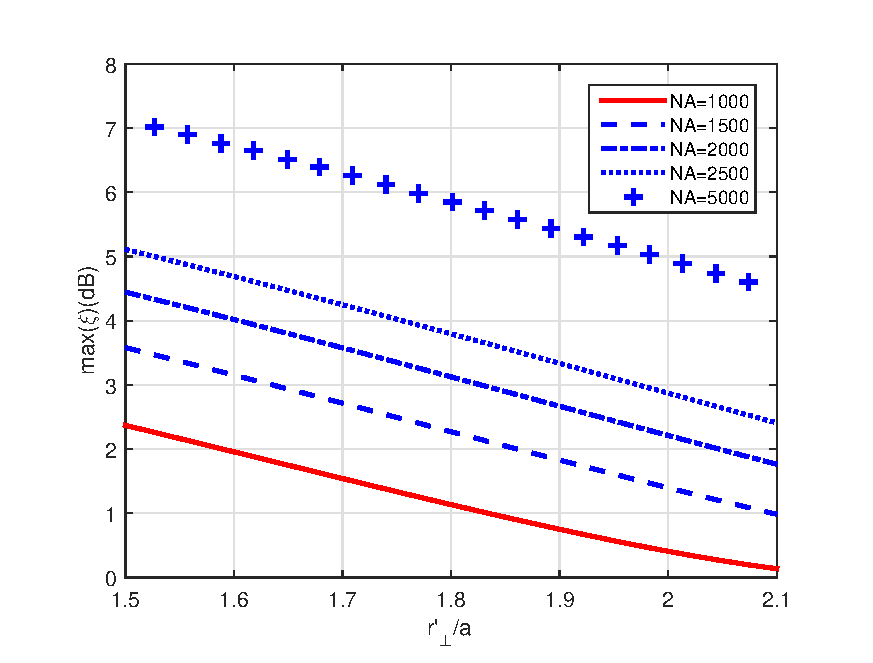
\includegraphics[scale=0.45]{./Figs/xi_optimal_NA1000to5000_omega44}}
%\end{minipage}
%\begin{minipage}{.49\linewidth}
%\centering
%\subfloat[]{\label{fig:OD_optimal_rp}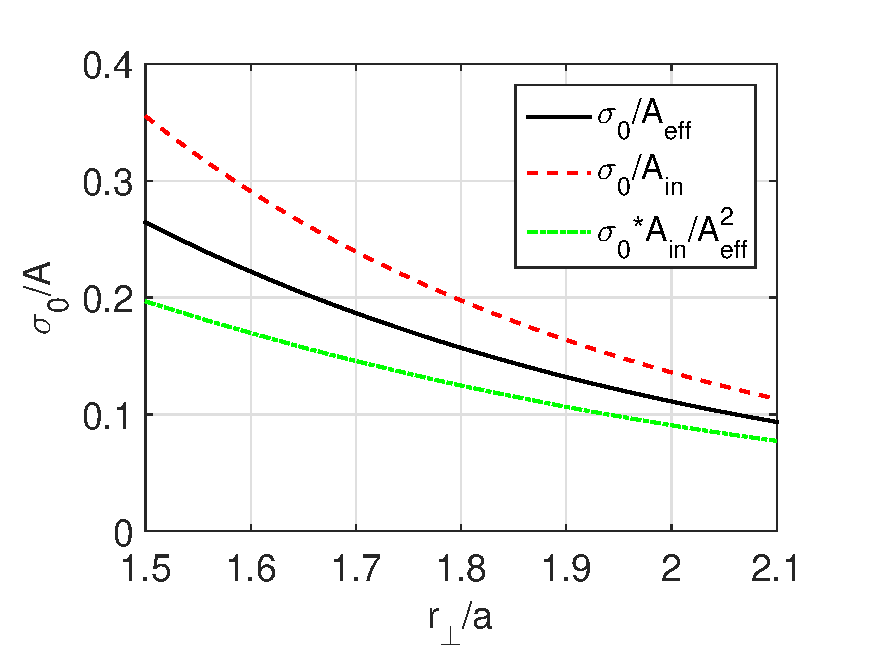
\includegraphics[scale=0.45]{./Figs/OD_optimal_rp}}
%\end{minipage}
%\caption{QND measurement properties using the magic frequency $ \omega_{44} $. Subfigure~\protect\subref{fig:xi_optimal_NA1000to5000_omega44} shows the optimal peak spin squeezing parameter as a function of the radial position of the atom. Different atom numbers have been indicated in different types of lines. Subfigure~\ref{fig:OD_optimal_rp} shows the OD per atom parameters and the ratio of $ \kappa/\gamma_s $ as a function of atoms' radial position when the optimal quantization axis is chosen to plot Subfig.~\protect\subref{fig:xi_optimal_NA1000to5000_omega44}.}\label{fig:QNDproperty_magic44}
%\end{figure}


\section{Relationship between OD/atom and cooperativity}
For atoms prepared in some state, the $\mathrm{OD}/\mathrm{atom}$ can be defined as
\begin{align}
\mathrm{OD}/\mathrm{atom} &= \frac{\sigma_0 }{A_{\rm eff} }, 
\end{align}
where the geometric property of the waveguide or optical medium and the inner structure property of the atoms have been absorbed into the effective mode area factor $ A_{\rm eff} $. 
While in cavity-QED, the concept of cooperativity is usually used to indicate the coupling strength between photons and atoms, and is equivalent to the cavity-to-free-space scattering ratio in the context of atomic cooling~\cite{Tanji-Suzukia2011,Vuletic2000,Kimble1998}. 
In this part, we want to show that the  $\mathrm{OD}/\mathrm{atom}$ in the context of traveling wave and atom interaction has an equivalent definition as the cooperativity in the context of optical cavity QED. 

Below, we consider a two-level atom interacting with an optical mode. 
From Eq.~\ref{Gamma1DGammavac_appendix} in the context of nanofiber geometry, we have
\begin{align}
\frac{\Gamma^{1\!D}}{\Gamma} &=   \frac{\sigma_0}{A_{\rm eff}}= \mathrm{OD}/\mathrm{atom}.
\end{align} 
The factor of $ \frac{1}{4} $ has been removed from Eq.~\ref{Gamma1DGammavac_appendix} when both propagating directions and polarizations of the modes are summed up in the equation above.

In the context of cavity-QED, the cooperativity per atom is defined as 
\begin{align}
C_1 &= \frac{2 g^2}{\kappa \Gamma},
\end{align}
where $ g=\frac{d\cdot E}{\hbar} $ is the coupling constant between the atom and the cavity mode with reduced dipole momentum $ \mathbf{d}=-e\bra{j}|\br|\ket{j'} $, and $ \kappa  $ and $ \Gamma $ are the decay rates of the cavity and atom respectively. 
One can use the relations that 
\begin{align}
E &= \sqrt{\frac{2\pi\hbar \omega}{V_{\rm eff}}}\\
V_{\rm eff} &= A_{\rm eff} L\\
\kappa &= \frac{c}{2L} \frac{1}{F}\\
\Gamma &= \frac{4}{3}\frac{\omega^3}{c^3} \frac{d^2}{\hbar}
\end{align}
where $ F $ is the cavity finesse.
The cooperativity can be then rewrite as
\begin{align}
C_1 &= \frac{4\pi d^2 \omega}{\hbar A_{\rm eff}L}\cdot  \frac{2L}{c}F \cdot \frac{3}{4} \frac{c^3}{\omega^3} \frac{\hbar}{d^2} = \frac{6\pi c^2}{\omega^2} \frac{1}{A_{\rm eff}} F\\
&= \frac{3\lambda^2}{2\pi} \frac{1}{A_{\rm eff}} F = \frac{\sigma_0}{A_{\rm eff}} F\\
&= \frac{\mathrm{OD}}{\mathrm{atom}} F.
\end{align}

For a Fabry–Pérot type cavity, the finesse is defined as the number of round trip a photon can make before leaking out, which only depends on the mirror reflectivity of the cavity. 
Alternatively, in terms of Q-factor, the finesse of a cavity can be written as $ F= Q\nu_F/\nu_0= Q \pi c/L\omega_0 $ with the Q-factor $ Q=\frac{\nu_0}{\delta\nu} $ and $ \nu_0 $ is the resonant frequency and $ \nu_F $ is the resonant frequency spacing~\cite{Saleh2007}. 
Giving a Gaussian mode with mode waist $ W_0 $, the cooperativity of an atom in the cavity becomes
\begin{align}
C_1 &= \frac{\sigma_0}{\pi W_0^2} F = \frac{\sigma_0}{A} F = \frac{\mathrm{OD}}{\mathrm{atom}} F.
\end{align}
This result agrees with literature~\cite{Hunger2010}. 

To increase the coupling strength between atoms and photons with a nanofiber, the atom number plays the role of cavity finesse in the context of optical cavity and relaxes the requirement of optical mode confinement in the dispersive regime. 

%</atomicphysicsformulas>

\bibliographystyle{../styles/abbrv-alpha-letters-links}
%\bibliographystyle{unsrt}
% \nocite{*}
\bibliography{../refs/Archive}

\printindex

\end{document}          